\documentclass[border=6pt,tikz]{standalone}
\usepackage{tikz}
\usepackage{amsmath,amssymb}
\usetikzlibrary{arrows.meta,positioning,fit,backgrounds,calc,shapes.geometric,decorations.pathreplacing,patterns}
\definecolor{ink}{HTML}{1B2430}
\definecolor{muted}{HTML}{6B7785}
\definecolor{accent}{HTML}{2F6FB5}
\definecolor{accent2}{HTML}{C1611F}
\definecolor{good}{HTML}{2E7D5B}
\definecolor{soft}{HTML}{EDF2F7}
\definecolor{soft2}{HTML}{FBEDE2}
\definecolor{soft3}{HTML}{E6F0E9}
\tikzset{
  box/.style={draw=ink,line width=.7pt,rounded corners=2pt,fill=soft,inner sep=4pt,align=center,font=\sffamily\small},
  boxa/.style={box,fill=soft2},
  boxb/.style={box,fill=soft3},
  plain/.style={align=center,font=\sffamily\small,text=ink},
  tiny/.style={align=center,font=\sffamily\scriptsize,text=muted},
  ar/.style={-{Stealth[length=2.4mm]},draw=ink,line width=.7pt},
  arm/.style={-{Stealth[length=2.4mm]},draw=muted,line width=.6pt,dashed},
  nd/.style={circle,draw=ink,line width=.7pt,fill=white,minimum size=7mm,inner sep=0pt,font=\sffamily\scriptsize},
  ndf/.style={nd,fill=soft},
  ndt/.style={nd,fill=soft2},
}

\tikzset{mine/.style={circle,fill=ink,minimum size=4.2mm,inner sep=0pt},
  his/.style={circle,draw=ink,line width=.8pt,fill=white,minimum size=4.2mm,inner sep=0pt},
  hole/.style={fill=muted!75},
  lab/.style={font=\sffamily\scriptsize,text=ink,inner sep=0pt}}
\definecolor{me}{HTML}{CFE0F3}\definecolor{him}{HTML}{F6D9C3}\definecolor{neutral}{HTML}{E4E7EB}
\begin{document}
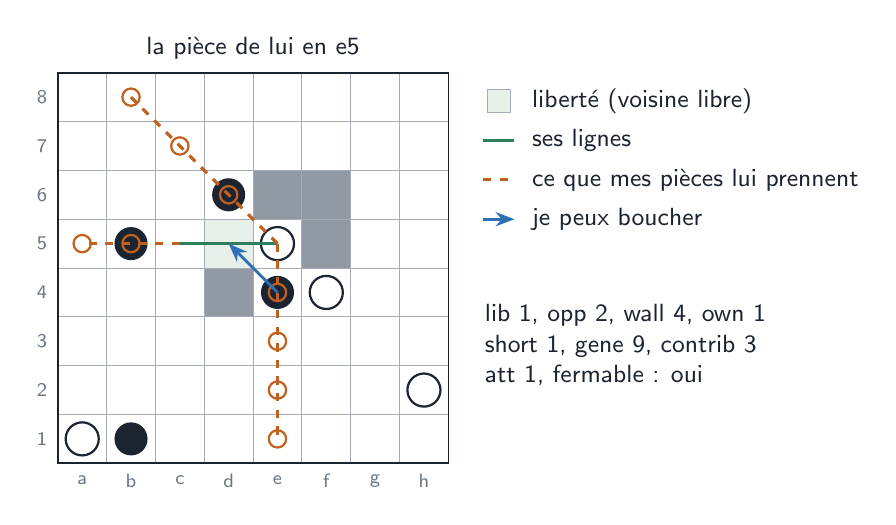
\begin{tikzpicture}
\begin{scope}[shift={(0.00,0)}]
\fill[soft3] (1.860,2.480) rectangle +(0.620,0.620);
\fill[white] (3.100,2.480) rectangle +(0.620,0.620);
\fill[white] (1.860,3.100) rectangle +(0.620,0.620);
\fill[white] (2.480,3.100) rectangle +(0.620,0.620);
\fill[white] (3.100,3.100) rectangle +(0.620,0.620);
\fill[white] (1.860,1.860) rectangle +(0.620,0.620);
\fill[white] (2.480,1.860) rectangle +(0.620,0.620);
\fill[white] (3.100,1.860) rectangle +(0.620,0.620);
\fill[hole] (1.860,1.860) rectangle +(0.620,0.620);
\fill[hole] (3.100,2.480) rectangle +(0.620,0.620);
\fill[hole] (2.480,3.100) rectangle +(0.620,0.620);
\fill[hole] (3.100,3.100) rectangle +(0.620,0.620);
\draw[muted!60,line width=.3pt,step=0.62] (0,0) grid (4.960,4.960);
\draw[ink,line width=.6pt] (0,0) rectangle (4.960,4.960);
\node[mine] at (0.930,2.790) {};
\node[mine] at (2.170,3.410) {};
\node[mine] at (2.790,2.170) {};
\node[mine] at (0.930,0.310) {};
\node[his] at (0.310,0.310) {};
\node[his] at (2.790,2.790) {};
\node[his] at (3.410,2.170) {};
\node[his] at (4.650,0.930) {};
\node[tiny] at (0.310,-0.22) {a};
\node[tiny] at (0.930,-0.22) {b};
\node[tiny] at (1.550,-0.22) {c};
\node[tiny] at (2.170,-0.22) {d};
\node[tiny] at (2.790,-0.22) {e};
\node[tiny] at (3.410,-0.22) {f};
\node[tiny] at (4.030,-0.22) {g};
\node[tiny] at (4.650,-0.22) {h};
\node[tiny] at (-0.2,0.310) {1};
\node[tiny] at (-0.2,0.930) {2};
\node[tiny] at (-0.2,1.550) {3};
\node[tiny] at (-0.2,2.170) {4};
\node[tiny] at (-0.2,2.790) {5};
\node[tiny] at (-0.2,3.410) {6};
\node[tiny] at (-0.2,4.030) {7};
\node[tiny] at (-0.2,4.650) {8};
\node[plain,above] at (2.480,5.010) {la pièce de lui en e5};
\end{scope}
\begin{scope}[shift={(0.00,0)}]\draw[accent2,line width=1.1pt,dashed] (2.790,2.790) -- (2.790,0.310);\node[circle,draw=accent2,line width=.8pt,minimum size=2.2mm,inner sep=0pt] at (2.790,2.170) {};\node[circle,draw=accent2,line width=.8pt,minimum size=2.2mm,inner sep=0pt] at (2.790,1.550) {};\node[circle,draw=accent2,line width=.8pt,minimum size=2.2mm,inner sep=0pt] at (2.790,0.930) {};\node[circle,draw=accent2,line width=.8pt,minimum size=2.2mm,inner sep=0pt] at (2.790,0.310) {};\draw[good,line width=1.1pt] (2.790,2.790) -- (1.550,2.790);\draw[accent2,line width=1.1pt,dashed] (1.550,2.790) -- (0.310,2.790);\node[circle,draw=accent2,line width=.8pt,minimum size=2.2mm,inner sep=0pt] at (0.930,2.790) {};\node[circle,draw=accent2,line width=.8pt,minimum size=2.2mm,inner sep=0pt] at (0.310,2.790) {};\draw[accent2,line width=1.1pt,dashed] (2.790,2.790) -- (0.930,4.650);\node[circle,draw=accent2,line width=.8pt,minimum size=2.2mm,inner sep=0pt] at (2.170,3.410) {};\node[circle,draw=accent2,line width=.8pt,minimum size=2.2mm,inner sep=0pt] at (1.550,4.030) {};\node[circle,draw=accent2,line width=.8pt,minimum size=2.2mm,inner sep=0pt] at (0.930,4.650) {};\draw[ar,accent,line width=1pt] (2.790,2.170) -- (2.170,2.790);\end{scope}
\begin{scope}[shift={(0.00,0)}]\begin{scope}[shift={(5.60,4.60)}]\fill[soft3] (-0.15,-0.15) rectangle (0.15,0.15);\draw[muted!60,line width=.3pt] (-0.15,-0.15) rectangle (0.15,0.15);\node[plain,right] at (0.3,0) {liberté (voisine libre)};\end{scope}
\begin{scope}[shift={(5.60,4.10)}]\draw[good,line width=1.1pt] (-0.2,0) -- (0.2,0);\node[plain,right] at (0.3,0) {ses lignes};\end{scope}
\begin{scope}[shift={(5.60,3.60)}]\draw[accent2,line width=1.1pt,dashed] (-0.2,0) -- (0.2,0);\node[plain,right] at (0.3,0) {ce que mes pièces lui prennent};\end{scope}
\begin{scope}[shift={(5.60,3.10)}]\draw[ar,accent,line width=1pt] (-0.2,0) -- (0.2,0);\node[plain,right] at (0.3,0) {je peux boucher};\end{scope}\end{scope}
\begin{scope}[shift={(0.00,0)}]\node[plain,right,align=left] at (5.3,1.5) {lib 1, opp 2, wall 4, own 1\\short 1, gene 9, contrib 3\\att 1, fermable : oui};\end{scope}
\end{tikzpicture}
\end{document}
